\subsection{Learning Pipeline}
\subsubsection{Learning Tasks}
Several behaviours were witnessed throughout data collection that pose interesting learning challenges for users of this dataset. By only providing the end effector position, no information is explicitly provided about the curvature of the robot. Cases arise where the robot can take on different shapes given the same end effector position by making use of the external forces applied on the end effector. An example of this is shown in Figure \ref{fig:multiple_solutions}. The two arms shown would have different dynamic behaviour during operation and so it may be valuable to have systems that have state representations larger than just an end effector position. This idea is what motivated the use of a larger LSTM layer in the learning-based controller state estimation sub-model. 

\begin{figure}[h]
    \centering
    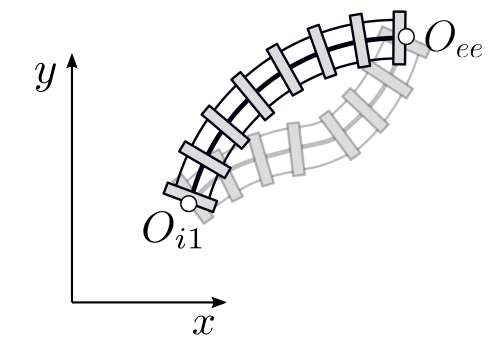
\includegraphics[width=0.5\textwidth]{images/multiple_solutions.png}
    \caption{Example of two robot configurations with equal tendon displacements}
    \label{fig:multiple_solutions}
\end{figure}

Another behaviour relating to the tendon slack issue discussed in Section \ref{sec:prototype_limitations_discussion} is exacerbated in the dataset because of the beam spring effect. When the robot's arm is being contracted, a restoring force acts on the end effector. If this restorative force is large enough, when the robot switches between contracting and extension the end effector will jump slightly to achieve tension in the tendon on the other side of the arm. For this to happen, the restorative force must be great enough to overcome static friction between the end effector and the table. This behaviour can be very sudden and is what results in the significantly higher maximum velocity during robot extension. When the restoring force is not great enough to overcome static friction, a period of time will pass where the motor is actuated with no end effector motion. There are only certain states that allow for this stationary behaviour to occur and it is not clear how to explicitly find them, they are not solely related to end effector position. Figure \ref{fig:equillibrium_position} shows one such equilibrium state. 

\begin{figure}[h]
    \centering
    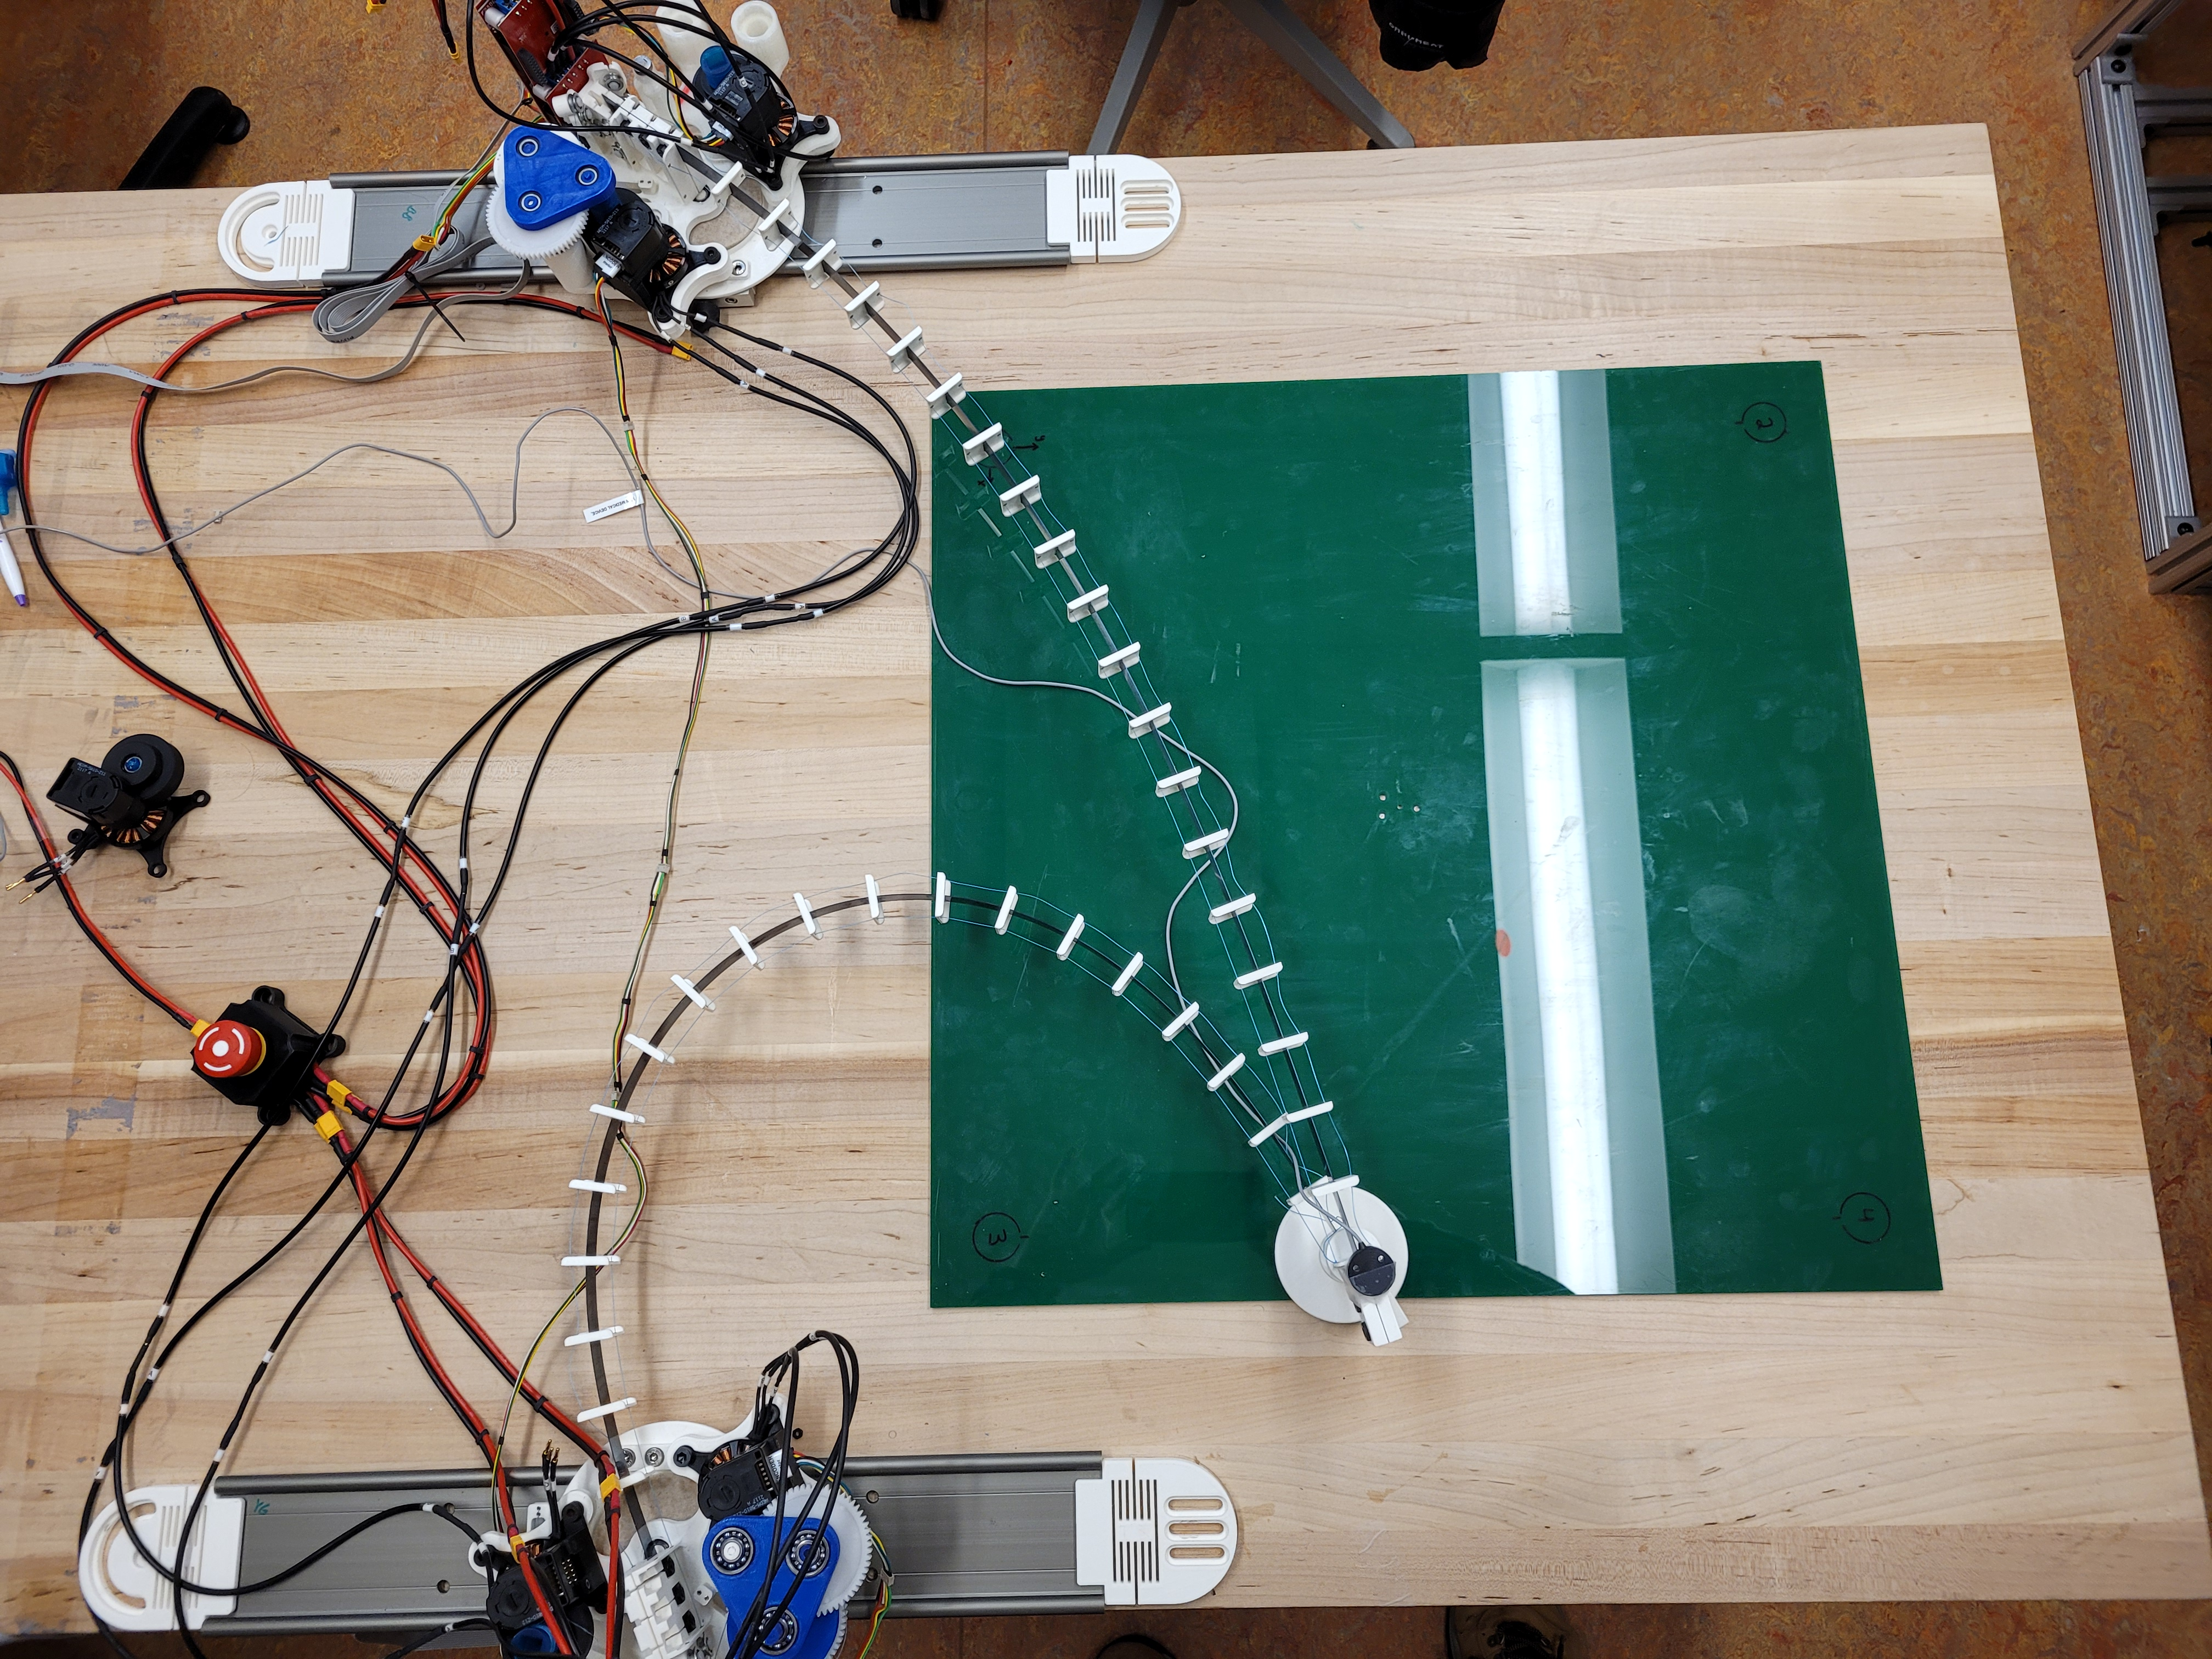
\includegraphics[width=0.5\textwidth]{images/equillibrium_location.jpg}
    \caption{Example of an equilibrium position where the robot will remain stationary despite motor actuation}
    \label{fig:equillibrium_position}
\end{figure}

\subsubsection{Expected Impact}
Learning-based approaches have the potential to model arbitrarily complex dynamic systems. Using this dataset, the expectation is that learning-based controllers will greatly improve upon the baseline accuracy. This is especially true when the model is moving fast or bending far, where the baseline model assumptions are less accurate. These models will be able to more accurately estimate the system kinematics and dynamics, enabling real-time tracking in task space for this robot. 

While there does not exist a direct comparison in the literature to the proposed parallel planar system, several references suggest that accuracy results in the range of 0.5-2\% of the robot's length could be expected with further controller development \cite{grassmann2022a, 7112506, 10.3389/frobt.2021.730330}. As this is the first step towards learning-based control being proposed for a PCR, accuracy comparable with current state-of-the-art for other CRs is only useful to provide a ballpark of what is possible. 